
\begin{frame}
    \begin{center}
        \LARGE 工作进展
    \end{center}
\end{frame}

\newsavebox{\BADGERScript}
\begin{lrbox}{\BADGERScript}
\begin{lstlisting}
$ python bes-dirac-dms-get-lfn-by-query-meta.py bossVer=6.5.5
/BES3/File/psipp/6.5.5/data/all/exp1/run_0011429_All_file015_SFO-1
/BES3/File/psipp/6.5.5/data/all/exp1/run_0011429_All_file015_SFO-2
/BES3/File/psipp/6.5.5/data/all/exp1/run_0011429_All_file016_SFO-1
...
$ python bes-dirac-dms-get-lfn-by-dataset.py --help
\end{lstlisting}
\end{lrbox}

\begin{frame}
    \frametitle{DIRAC方面}
    \begin{itemize}
        \item 投入时间较少。由于整个框架较为复杂,大多数时间在研究代码。
        \item 布置的任务主要在数据传输。
            \begin{itemize}
                \item 真正的传输还未实现。
                \item 已实现根据查询条件,给出满足需要的文件列表。
                \item 代码存放:\url{https://github.com/mirguest/MirguestIssueReport/tree/master/DIRAC/BES/BADGER/DataTransfer/scripts}
            \end{itemize}
    \end{itemize}
    \begin{block}{例子}
        \par\usebox{\BADGERScript}
    \end{block}
\end{frame}

\begin{frame}
    \frametitle{DIRAC方面(续)}
    \begin{itemize}
        \item 国庆期间,为DIRAC File Catalog CLI添加自动补全功能
        \item 在github上,发送了两次pull request。已全部接受。
    \end{itemize}
    \begin{block}{发送的Pull Request}
        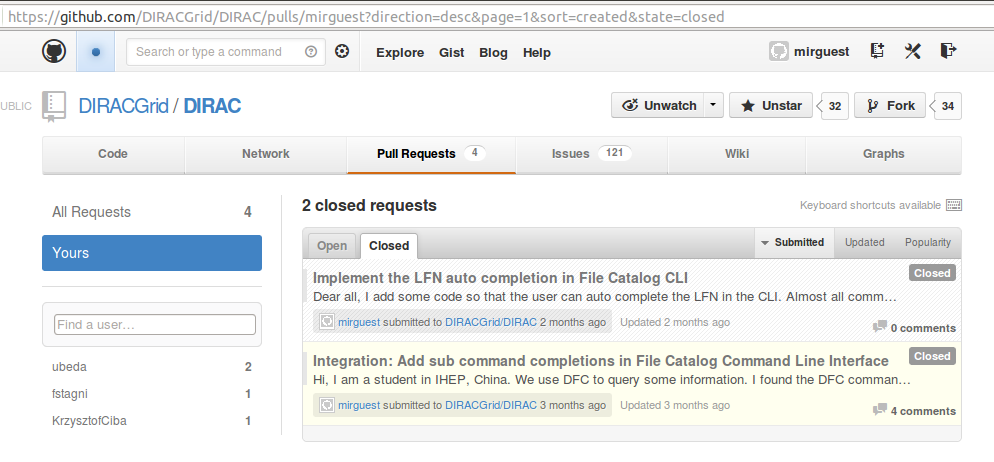
\includegraphics[height=5cm,keepaspectratio]{data/dirac_pull_request.png}
    \end{block}
\end{frame}

\begin{frame}
    \frametitle{大亚湾二期方面的工作}
    \begin{itemize}
        \item 初步搭建二期模拟软件的环境
            \begin{columns}
                \column{4.0cm}
                    \begin{itemize}
                        \item 开发时需要的软件及库
                        \item Geant4 9.4, 9.5, 9.6
                        \item ROOT
                        \item CLHEP
                        \item CERNLIB
                        \item curl
                        \item git
                    \end{itemize}
                \column{6.0cm}
                    \begin{itemize}
                        \item 服务器的管理
                        \item \url{dyb2app1.ihep.ac.cn}
                        \item gitolite
                        \item Trac
                        \item 目前作为管理员,对代码访问及开发进行授权
                    \end{itemize}
            \end{columns}
        \item 做过一次tutorial。\url{http://dyb2app1.ihep.ac.cn/trac/attachment/wiki/StartGameChineseVersion/tracgit.pdf}
    \end{itemize}
\end{frame}

\begin{frame}
    \frametitle{反射光锥的研究}
    \begin{itemize}
        \item 指导老师:何苗
        \item 主要工作:
            \begin{itemize}
                \item 参考何苗的光锥构造代码,编写新的光锥构造代码
                \item 可在运行时控制光锥几何大小。便于研究锥高对PMT吸收率的影响。
                \item 开始使用git来管理代码,在自己电脑上,搭建gitosis+Trac管理代码。
                \item 将代码迁移至Geant4 9.4。但Low Energy部分未迁移。
                \item 此处,使用8inch PMT。
            \end{itemize}
    \end{itemize}
\end{frame}

\begin{frame}
    \frametitle{反射光锥,平面摆放}
    \begin{columns}
        \column{5.0cm} 
            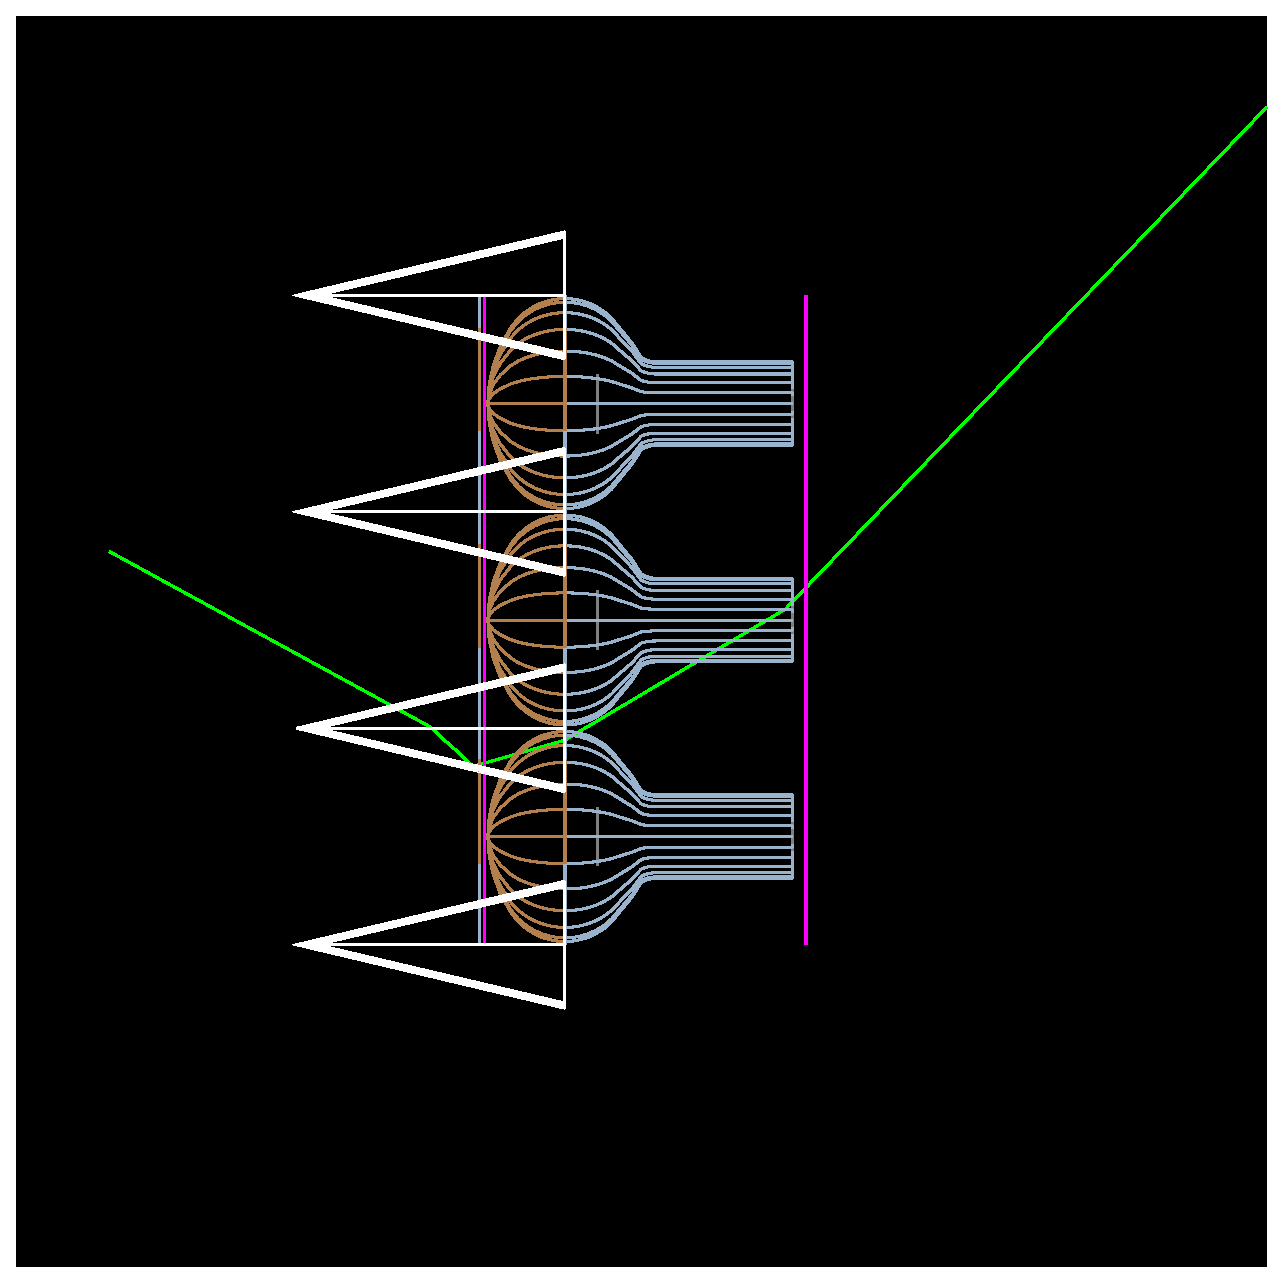
\includegraphics[height=5cm, keepaspectratio]{data/OptTrd_0.eps}
        \column{5.0cm} 
            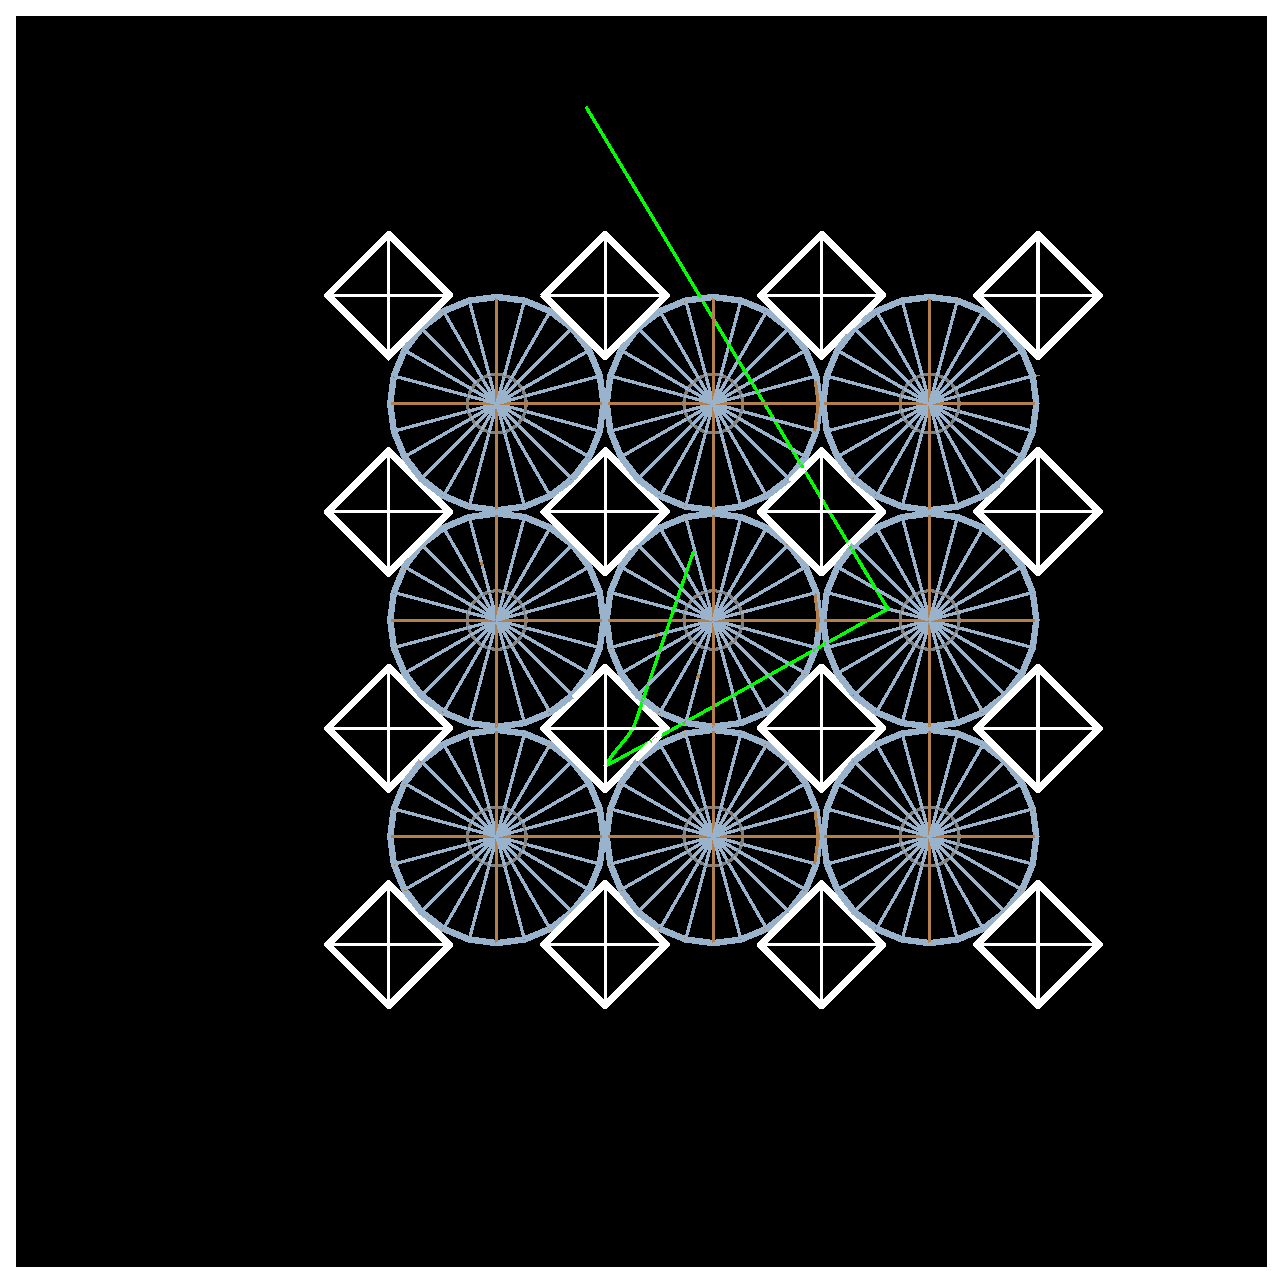
\includegraphics[height=5cm, keepaspectratio]{data/OptTrd_1.eps}
    \end{columns}
\end{frame}

\begin{frame}
    \frametitle{反射光锥,平面摆放,9x9阵列,扫描入射角,锥高}
    \begin{columns}
        \column{5.0cm} 
            光子收集效率

            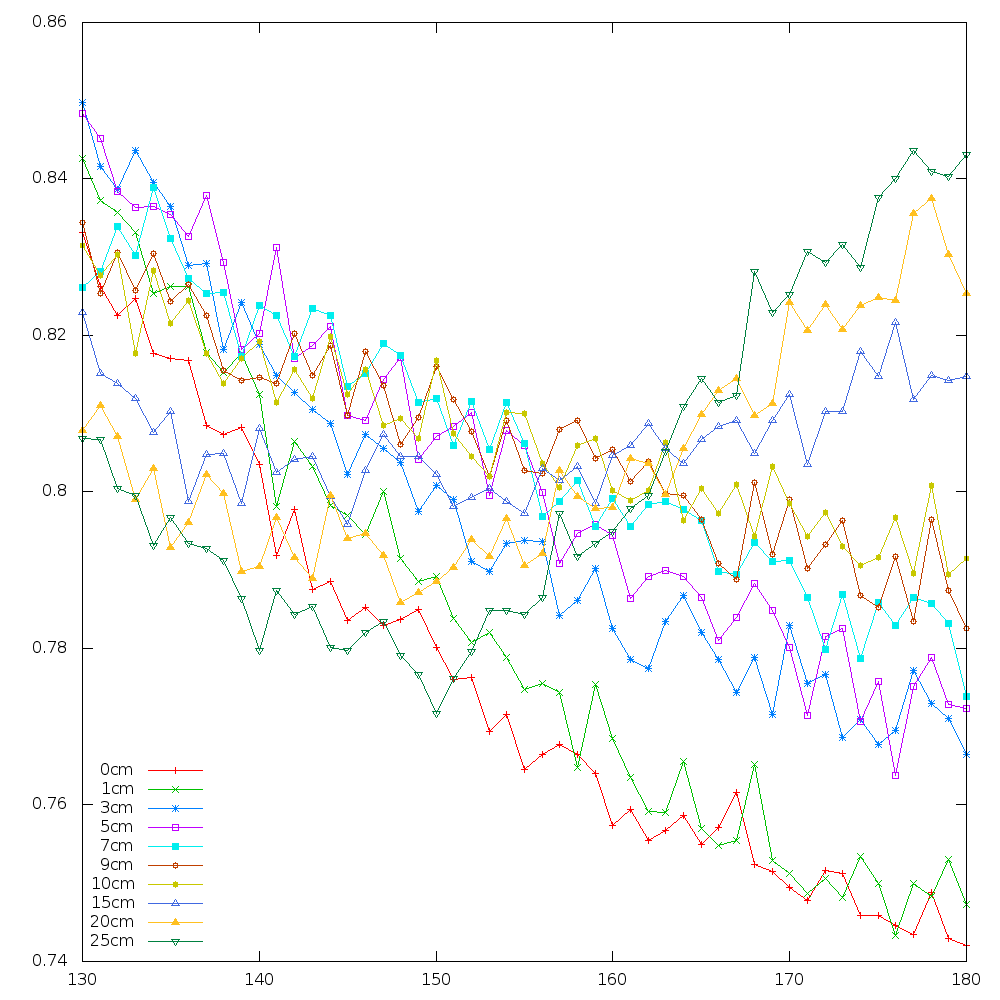
\includegraphics[height=5cm, keepaspectratio]{data/opttrd_incient_theta.png}
        \column{5.0cm} 
            相对没有反射锥的效率变化

            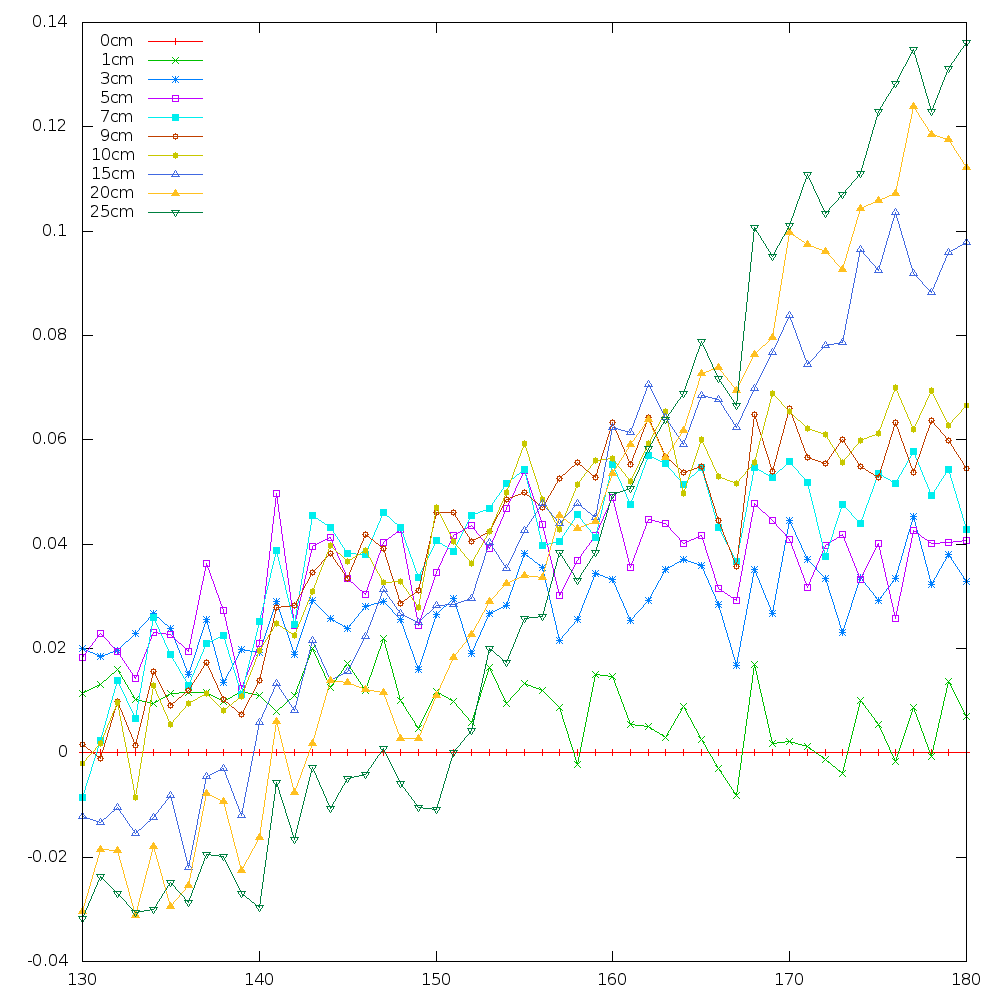
\includegraphics[height=5cm, keepaspectratio]{data/opttrd_incient_theta_rel.png}
    \end{columns}
\end{frame}

\begin{frame}
    \frametitle{反射光锥,柱型摆放}
    \begin{columns}
        \column{7.0cm} 
            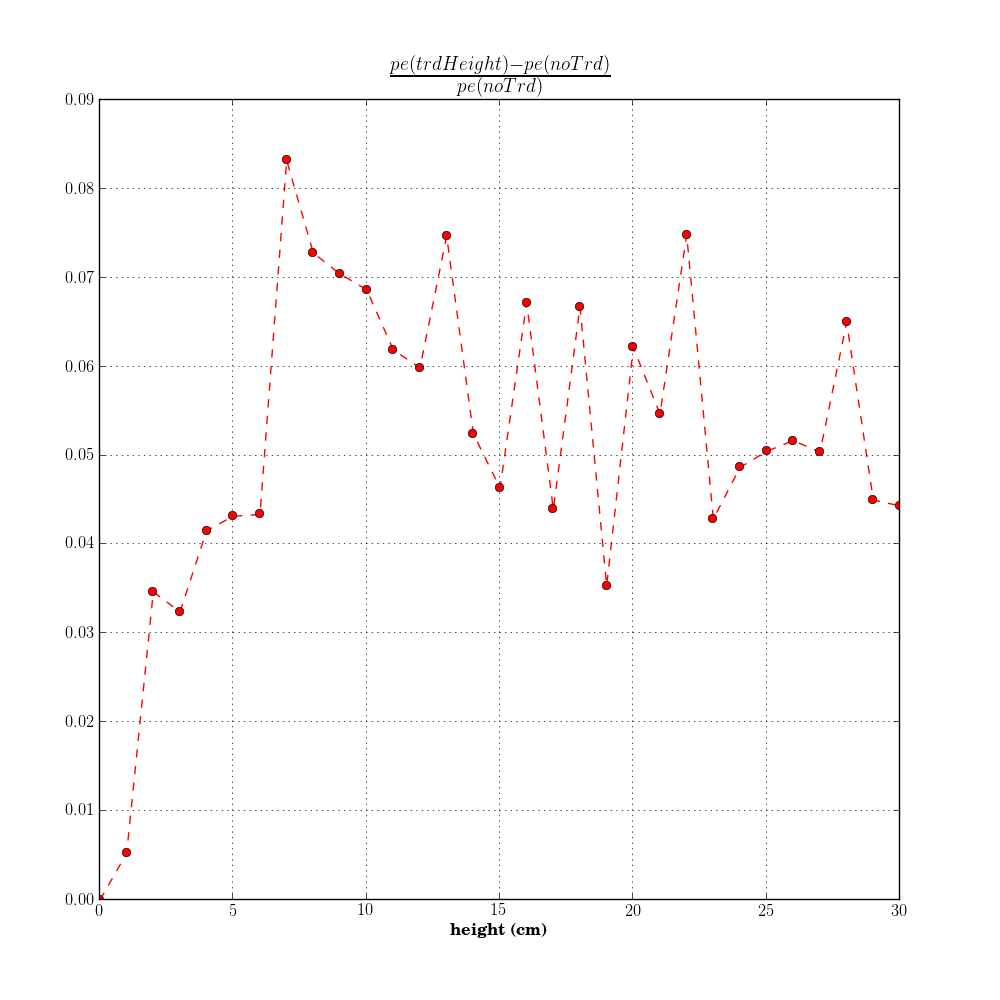
\includegraphics[height=7cm, keepaspectratio]{data/tube_full_random.png}
        \column{4.0cm} 
            \begin{itemize}
                \item 探测器为液闪+有机玻璃罐+油。
                \item 8inch PMT
                \item 顶部,底部为正方阵列,151*151;
                \item 柱面:一圈501个PMT,沿z向有145圈;
                \item 摆放半径为17m,高度31m。
            \end{itemize}
    \end{columns}
\end{frame}

\begin{frame}
    \frametitle{中心探测器初步研究:LS+Water}
    \begin{itemize}
        \item 指导老师:邓子艳
        \item 主要工作:
            \begin{itemize}
                \item 能量分辨率的研究
                \item PMT位置的摆放算法,解决原来球形几何中PMT重叠的问题。
                \item PMT从8inch到20inch过渡。
                \item 添加几种控制命令(可参考代码中的mac文件),
                      可在球面,球体内产生,并可混入多种粒子。
                \item 开始使用github提供的issue功能,记录软件开发时的各种问题。
            \end{itemize}
    \end{itemize}
\end{frame}

\begin{frame}
    \frametitle{PMT摆放}
    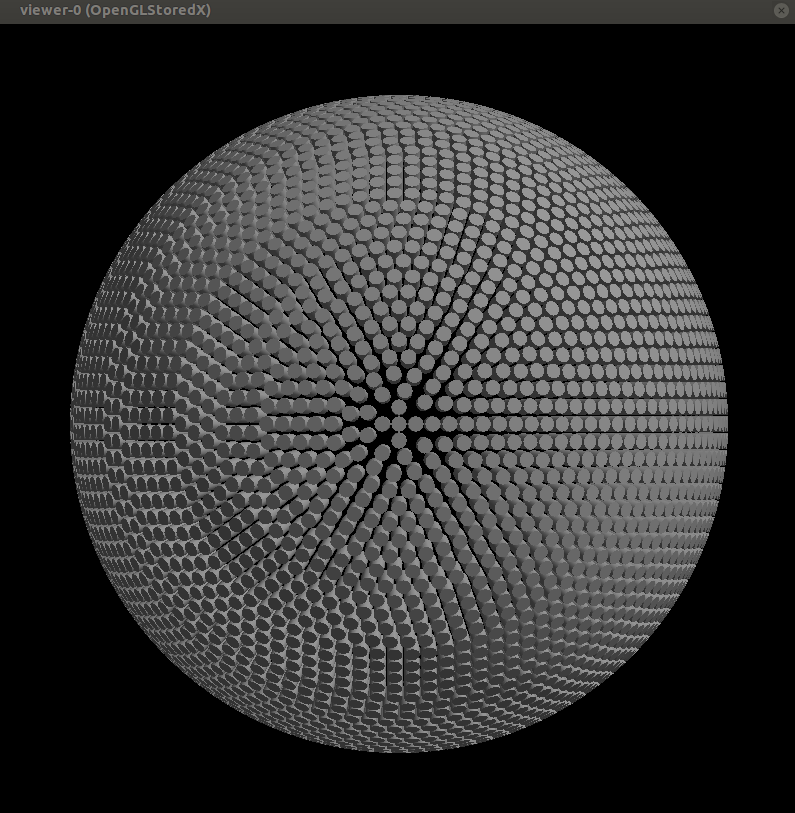
\includegraphics[height=8cm,keepaspectratio]{data/pmts_in_ball.png}
\end{frame}

\begin{frame}
    \frametitle{使用github的issue功能}
        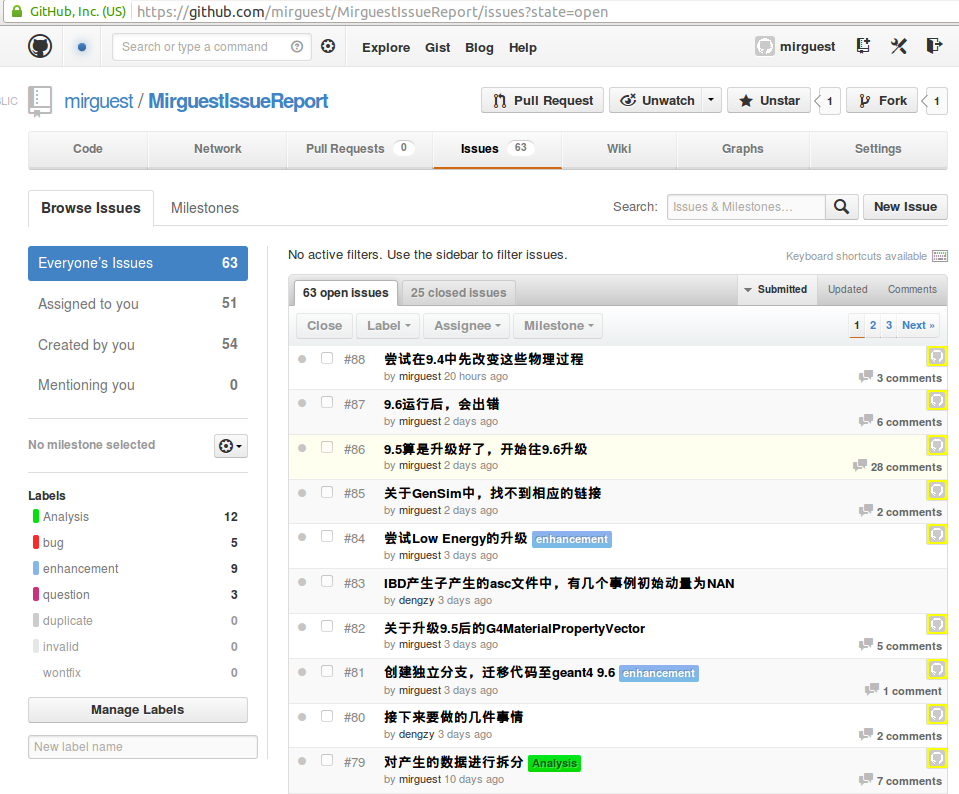
\includegraphics[height=8cm,keepaspectratio]{data/github_issue_own.png}
\end{frame}

% LS 

\begin{frame}
    \frametitle{中心探测器方案六研究:LS}
    \begin{itemize}
        \item 指导老师:邓子艳
        \item 主要工作:
            \begin{itemize}
                \item 代码的整理。根据需求,把代码划分至几个模块之中。
                \item 能量分辨率的研究
                \item 引入U,Th,K及IBD产生子,解析HepEvt文件。
                \item 事例的拆分与合并。根据事例率按泊松分布进行抽样合并。
                \item 在PMT的玻璃上产生放射性本底事例。
                \item 尝试升级代码至9.5及9.6。
                \item Low Energy的迁移基本完成。在占亮的帮助下,
                      发现迁移后存在的一个bug:质子一直处于低能散射。
                      新版本下质子等的电离过程需要单独指明。
            \end{itemize}
    \end{itemize}
\end{frame}

\newsavebox{\BackgroundTest}
\begin{lrbox}{\BackgroundTest}
\begin{lstlisting}[language=C++]
const Int_t pmt_total = 14159;
static Int_t pmt[pmt_total];
Background* U = new Background("MC-U.root", 0.2 * 1.936/3.3);
Background* Th = new Background("MC-Th.root", 0.2 * 0.989/3.3);
Background* K = new Background("MC-K.root", 0.2 * 0.3748/3.3);     

for(Int_t i=0; i < 50000; ++i) {
    // Clear pmt;
    for(Int_t clearindex=0; clearindex<pmt_total; ++clearindex) {
        pmt[clearindex] = 0;
    }
    mix_entries = 0;
    mix_entries += U->yieldOneEntry(pmt);
    mix_entries += Th->yieldOneEntry(pmt);
    mix_entries += K->yieldOneEntry(pmt);
    total_pe = std::accumulate(pmt, pmt+pmt_total, 0);
}

\end{lstlisting}
\end{lrbox}

\begin{frame}
    \frametitle{本底混合的代码}
    \par\usebox{\BackgroundTest}
\end{frame}

\begin{frame}
    \frametitle{在一个玻璃上产生事例}
        %\includegraphics[height=8cm,keepaspectratio]{data/}
\end{frame}

% The other works.

\newsavebox{\ZhangYaoBossScript}
\begin{lrbox}{\ZhangYaoBossScript}
\begin{lstlisting}
$ cat ~/.bossrc 
[663]
boss = 6.6.2.p01
cmthome = /ihepbatch/bes/zhangyao/.cmthome663/
TestRelease = ~/work/663/TestRelease/TestRelease-00-00-79/cmt/setup.csh

[662]
boss = 6.6.2
cmthome = /ihepbatch/bes/zhangyao/.cmthome662/
TestRelease = ~/work/662/TestRelease/TestRelease-00-00-78/cmt/setup.csh
$ ./bosstest (*@{\color{red} -r 663}@*) -q sth
\end{lstlisting}
\end{lrbox}

\begin{frame}
    \frametitle{其他的一些工具:Boss作业提交工具}
    \begin{itemize}
        \item 指导老师:张瑶
        \item 工具简介:
            \begin{itemize}
                \item 在boss某版本下,提交其他版本的boss作业
                \item 用户只需在一个配置文件中指明版本号及cmthome等。
                \item 提交时只需要指明配置文件中的标签。
                \item 修改基于原来的boss脚本。
                \item 代码位于:\url{https://github.com/ihepzhangyao/script}
            \end{itemize}
    \end{itemize}
    \begin{block}{例子(排版所需,对内容有些修改)}
        \par\usebox{\ZhangYaoBossScript}
    \end{block}
\end{frame}
